\pdfoutput=1
% DRAFT PREAMBLE: quantumarticle.cls (GitHub master and TeX Live 2025) is
% currently incompatible with the 2025 LaTeX kernel on this machine
% ("Sorting rule for 'begindocument' hook applied too late"). Drafting with
% the article class; swap to quantumarticle at submission (e.g., on Overleaf
% with TeX Live <= 2023). See template/README.md.
\documentclass[a4paper,11pt]{article}
\usepackage[margin=2.2cm]{geometry}
\usepackage[utf8]{inputenc}
\usepackage[english]{babel}
\usepackage[T1]{fontenc}
\usepackage{amsmath,amssymb,amsthm}
\usepackage{graphicx}
\usepackage{hyperref}
\usepackage{booktabs}
\usepackage{authblk}
\usepackage{tikz}
\usetikzlibrary{positioning,arrows.meta}
\newcommand{\affiliation}[1]{\affil{#1}}

\newtheorem{theorem}{Theorem}
\newtheorem{observation}{Observation}

\newcommand{\tc}{\ensuremath{\mathrm{tc}}}
\newcommand{\sct}{\ensuremath{\mathrm{sc}}}
\newcommand{\scT}{\ensuremath{\mathrm{sc}_{\mathrm{target}}}}

\title{Certified frontiers for tensor-network contraction ordering}

\author{Jinguo Liu}
\affiliation{Advanced Materials Thrust, The Hong Kong University of Science and Technology (Guangzhou)}

\begin{document}
\maketitle

\begin{abstract}
Contraction-order optimizers for tensor networks are routinely compared
against each other, but almost never against certified references, so it is
unknown whether reported improvements approach any fundamental limit. We
carry out such a study on two closed benchmark networks---a 250-tensor
random 3-regular graph and a 561-tensor Sycamore-like random-circuit
proxy---under a fixed protocol: 90-second single-threaded budgets,
independent rescoring of every contraction tree from its topology, and
adversarial validation. We report three results. First, the single largest
practical lever we find is a mis-set default: annealing toward an
aspirationally low memory target ($\scT=20$) costs $4.3$ and $9.7$ in
$\log_2$ flops on the two instances ($20\times$ and $800\times$),
and simply removing the target recovers the entire loss; thirteen
mechanically distinct search mechanisms, implemented and scored under the
same protocol, recover nothing further. Second, the resulting frontier is
reproduced independently by cotengra's simulated-annealing refiner, while
its hyper-optimization mode remains $1.7$--$2.4$ behind at equal budget;
the frontier is also budget-independent over a $10\times$ range. Third, we
localize the optimum: on the circuit proxy the frontier is provably
width-optimal and the true minimum lies in $[53, 61.544]$; we prove two
sum-form lower bounds on the log-sum contraction cost and show that they,
and every bound computable from the isoperimetric profile alone, are capped
at the bisection width---an impossibility result explained by an explicit
low-boundary cut certificate and by a measured conservation-like behavior
of frontier cost profiles. All claims carry machine-checkable certificates
or full audit trails from the 31-attempt autonomous research loop that
produced them, which caught three distinct illusory-gain modes along the
way.
\end{abstract}


\section{Introduction}
\label{sec:intro}

The cost of contracting a tensor network is governed by the order in which
its tensors are combined. Finding a good order is the computational
bottleneck of classical random-circuit simulation
\cite{markov_2005_simulating, liu_2022_verifying}, and a rich ecosystem of
optimizers has grown around the problem: simulated-annealing refiners
\cite{kalachev_2021_multi}, hyper-optimized portfolios over greedy and
hypergraph-partitioning constructions \cite{gray_2020_hyper,
staudt_2024_improved}, treewidth machinery imported from the
parameterized-algorithms community \cite{dumitrescu_2018_benchmarking,
tamaki_2017_positive}, and exact methods for small networks
\cite{pfeifer_2013_faster}. These tools are compared against each other,
on wall-clock budgets, and the field's implicit quality standard is
relative: an optimizer is good if it beats another optimizer.

This paper asks the absolute questions. On fixed benchmark instances and a
fixed time budget: (i) how much of the attainable quality do shipped
defaults throw away; (ii) where do all known search paradigms actually
converge; and (iii) how far is that convergence point from the true
optimum---and can the gap be certified rather than conjectured?

We answer all three on two closed networks under a hardened evaluation
protocol (Sec.~\ref{sec:setup}). The answers are summarized in
Figs.~\ref{fig:sweep}--\ref{fig:bounds}: a mis-set default memory target
dominates every algorithmic effect we could produce
(Sec.~\ref{sec:sctarget}); thirteen search mechanisms and two independent
toolchains converge to a single frontier (Sec.~\ref{sec:frontier}); and
that frontier is provably width-optimal, with the optimum localized to a
certified interval whose residual resists an entire family of lower-bound
techniques for a reason we prove (Sec.~\ref{sec:bounds}). We close with
the behavior of the problem at larger scale (Sec.~\ref{sec:scale}) and
with the autonomous-loop methodology that produced---and repeatedly
corrected---these claims (Sec.~\ref{sec:method}).

\section{Setup and evaluation protocol}
\label{sec:setup}

\paragraph{Instances and cost model.}
A closed tensor network is a graph $G=(V,E)$: vertices are tensors, edges
are summed indices, and every index here has dimension~2. A contraction
order is a full binary tree whose leaves are the tensors; each internal
node $v$ contracts its two children into an intermediate tensor. Writing
$\mathrm{cost}_v$ for the $\log_2$ floating-point cost of node $v$ (the
sum of $\log_2$ dimensions over the union of the operands' indices), the
two standard quality measures are the total time cost
\begin{equation}
  \tc \;=\; \log_2 \sum_{v} 2^{\mathrm{cost}_v},
  \label{eq:tc}
\end{equation}
a log-sum-exp over all $|V|-1$ contractions, and the space cost $\sct$,
the $\log_2$ size of the largest intermediate. We use two instances
throughout: \emph{reg3\_250}, a random 3-regular graph with 250 tensors
and 372 indices, and \emph{sycamore\_m20}, a deterministic Sycamore-scale
random-quantum-circuit proxy with 561 tensors and 963 indices (53 qubits
on an $8\times 7$ grid minus three corners, 20 cycles of two-qubit gates
in the standard four-coloring pattern, contracted to a single amplitude).
We state explicitly that the latter is a structurally faithful proxy, not
the physical Sycamore circuit.

\paragraph{Protocol.}
Every optimizer run gets 90 seconds of single-threaded wall clock per
instance. Emitted trees are rescored by an independent checker that
recomputes $\tc$ and $\sct$ from the tree topology and the original index
sets alone; optimizer-reported numbers are never trusted. Instances are
randomly relabeled per run, so memorized answers keyed on input encoding
do not transfer. A best-known value (``record'') only moves when a run
beats it and a second run under fresh relabeling confirms; the worse of
the two runs is recorded. CPU-time accounting rejects hidden parallelism.
Reference rows are measured best-of-three with the identical pipeline.
The full validation harness, including its negative-control self-tests,
is described in Sec.~\ref{sec:method}.

\section{A mis-set default dominates all algorithmic effects}
\label{sec:sctarget}

The TreeSA-family annealers \cite{kalachev_2021_multi} optimize a
composite objective in which the space cost is pulled toward a target
$\scT$, with a penalty active whenever $\sct > \scT$. The
reference implementation we study (omeco, mirroring
OMEinsumContractionOrders.jl) ships $\scT = 20$.
On instances whose good trees have naturally larger intermediates---the
optimum-quality trees here have $\sct = 34$ and $53$---this default is not
merely unhelpful. It actively drags the search into a low-memory,
high-flop region of tree space.

Figure~\ref{fig:sweep} shows the resulting $\tc$ at a fixed 90-second
budget as a function of $\scT$. \textbf{This figure is our first main
result}, and the transition it reveals is a cliff, not a slope: every
target below the natural space cost of good trees is roughly equally
harmful (medians $45.6$--$47.0$ on reg3\_250, $71$--$77$ on
sycamore\_m20), quality snaps to the frontier exactly at the natural
value ($\scT = 34$ and $53$), and stays there unchanged through
$\scT=\infty$, i.e., with the memory objective deleted. The harm is
strictly one-directional. Two finer observations: targets just
\emph{below} the natural value are the worst on sycamore\_m20 (median
$77.0$ at $\scT=50$, versus $72.1$ at the shipped default of 20),
consistent with the penalty being most active precisely near the
boundary it cannot reach; and the natural-value target itself slightly
outperforms $\scT=\infty$ there ($61.51$ versus $61.67$, non-overlapping
ranges over three runs), so a correctly set finite target is never worse
than none. At the shipped default the damage is $4.3$ $\log_2$ units on
reg3\_250 and $9.7$ on sycamore\_m20: a $20\times$ and $800\times$ flop
overhead, recovered by a one-line change. An ablation within one of our
search mechanisms confirms the attribution: holding everything else
fixed and moving the penalty target to the natural space cost moved
reg3\_250 from $\tc=56.8$ to $40.0$, while that mechanism's novel
component contributed $0.002$.

The practical rule is: \emph{never anneal toward a memory target below
the natural space cost of good trees; absent a physical memory budget,
use the natural value or no target at all.} The corresponding fix
(default $\scT=\infty$, with finite values only when a real memory
budget is supplied) applies to omeco and, we expect, upstream
implementations sharing the default.

\begin{figure}[t]
  \centering
  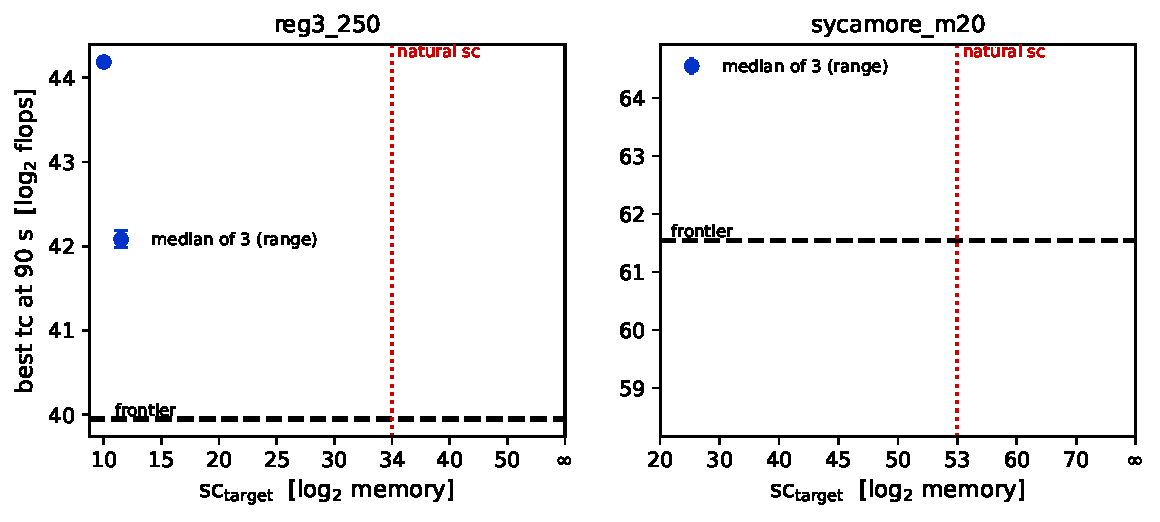
\includegraphics[width=\linewidth]{figures/fig1_sctarget_sweep.pdf}
  \caption{Best $\tc$ reached in 90\,s of single-threaded annealing versus
  the memory target $\scT$ (median of three runs; whiskers span the
  range). The dashed line marks the frontier value of
  Sec.~\ref{sec:frontier}; the dotted vertical line marks the natural
  space cost of optimum-quality trees. The transition is a cliff at the
  natural value: every smaller target is comparably harmful, and every
  target at or above it, including $\scT=\infty$, reaches the frontier.
  The shipped default is $\scT=20$.}
  \label{fig:sweep}
\end{figure}

\section{Thirteen mechanisms, two toolchains, one frontier}
\label{sec:frontier}

With the objective corrected, we attempted to beat the resulting
reference with mechanically distinct search paradigms, implemented
independently and scored under the protocol of Sec.~\ref{sec:setup}:
coarse subtree-transfer moves and basin hopping
\cite{anon_2025_optimizing}, evolutionary replica populations, exact-penalty
ramps through infeasible regions, tabu search with strategic oscillation,
large-neighborhood destroy-and-repair, beam search with lookahead,
Boltzmann-greedy portfolios \cite{gray_2020_hyper, orgler_2024_optimizing},
recursive balanced min-cut construction \cite{strasser_2017_computing,
staudt_2024_improved}, elimination-order annealing
\cite{dumitrescu_2018_benchmarking}, order-then-tree interval dynamic
programming \cite{ibrahim_2022_constructing}, hierarchical
coarsen-then-exact solves, structure-guided sweeps exploiting the
circuit's spacetime geometry, and profile-aware annealing
(Sec.~\ref{sec:bounds}).

Figure~\ref{fig:frontier} shows every scored result as its distance from
the best verified value. All thirteen mechanisms land within $0.35$
$\log_2$ of the corrected reference on both instances---most within
noise---and none set a confirmed record against it. The same frontier is
reproduced by an independent toolchain: cotengra's simulated-annealing
refiner \cite{gray_2020_hyper} ties it to within $0.05$ and $0.14$, while
cotengra's hyper-optimization mode alone (greedy and hypergraph
partitioning portfolios, without SA refinement) remains $1.7$ and $2.4$
behind at the same matched budget. The frontier is also
budget-independent: extending the budget tenfold, to 900 seconds, moves
it by less than $0.1$ (Fig.~\ref{fig:scale}a). We conclude that at this
scale the frontier is a property of the cost landscape, not of any
particular search mechanism, schedule, or implementation.

Two honest qualifications. First, these comparisons are matched-budget,
single-threaded, and slicing-free by design; cotengra's strengths in
massively parallel trial sampling and sliced contraction lie outside this
protocol. Second, convergence of many searchers is evidence of a shared
basin, not of optimality---which is precisely why certified bounds are
needed, and to which we now turn.

\begin{figure}[t]
  \centering
  
\includegraphics[width=\linewidth]{figures/fig2_frontier_convergence.pdf}
  \caption{Distance of every scored optimizer from the frontier value
  (dashed line at zero). Open triangles: the thirteen search mechanisms
  of this work. Filled symbols: the corrected TreeSA reference
  ($\scT=\infty$, circle), cotengra's SA refiner (diamond), cotengra's
  hyper-optimizer (square), and the shipped-default TreeSA (cross).}
  \label{fig:frontier}
\end{figure}

\section{Certified bounds: width-optimality, the interval, and an
impossibility result}
\label{sec:bounds}

\subsection{Max-form bounds and width-optimality of the frontier}

Every classical lower-bound technique for contraction cost is
\emph{max-form}: it bounds the single largest contraction. The
Markov--Shi correspondence \cite{markov_2005_simulating} equates the
minimal largest contraction rank with the treewidth of the line graph
$L(G)$, and any balanced edge of a contraction tree yields a cut whose
boundary lower-bounds the largest contraction.

On sycamore\_m20 these tools give a sharp result. An explicit temporal
cut severing all 53 qubit world-lines gives a balanced cut of value 53;
extensive search finds nothing smaller, and the frontier trees achieve
$\sct = 53$ exactly. The frontier is therefore \emph{width-optimal}: no
contraction tree of this network has a smaller largest intermediate, and
consequently $\mathrm{tw}(L(G)) = 52$. Combined with the frontier value,
\textbf{our second main result} is the certified localization
\begin{equation}
  \tc_{\min}(\text{sycamore\_m20}) \;\in\; [\,53,\; 61.544\,].
  \label{eq:interval}
\end{equation}
On reg3\_250, certifying the analogous statement is obstructed by the
known hardness of certifying high treewidth on expanders: the best
machine-verified certificate (a 32-vertex minor of $L(G)$, checked by two
independent exact solvers) gives $\mathrm{tw}(L(G)) \ge 18$ against a
constructive upper bound of 34, so the structural picture
$39.95 \approx 34 + \text{(log-sum overhead)}$ remains uncertified.

The width bound, however, has a ceiling: $\tc$ is a log-sum
\eqref{eq:tc} over $\sim\!|V|$ contractions, and the frontier's excess
over the width bound---$8.5$ on sycamore\_m20, close to the maximal
possible $\log_2 561 = 9.1$---is invisible to any bound on a single
contraction. Closing the interval \eqref{eq:interval} from below requires
\emph{sum-form} bounds.

\subsection{Sum-form bounds and their collapse}

For any tree, each internal node $v$ with leaf set $S_v$ satisfies
$\mathrm{cost}_v \ge |\partial S_v|$, the boundary of $S_v$ in $G$.
Writing $b(k)$ for the isoperimetric profile of $G$ (the minimal boundary
over all $k$-vertex subsets), we prove:

\begin{theorem}[Sum-form profile bound]
\label{thm:sum}
For every contraction tree,
$\tc \ge \log_2 F(n)$ where $F$ obeys the recursion
$F(1)=0$, $F(k) = 2^{\,b(k)} + \min_{1\le j\le k/2}\,[F(j)+F(k-j)]$.
\end{theorem}

\begin{theorem}[Dyadic-window bound]
\label{thm:window}
Descending from the root always into the larger child visits, for every
dyadic window $W_j = (n/2^{j+1}, n/2^{j}]$, at least one internal node
whose leaf-set size lies in $W_j$; these nodes are distinct, hence
$\tc \ge \log_2 \sum_j 2^{\,\min_{k \in W_j} b(k)}$.
\end{theorem}

Both theorems are validated computationally (exhaustively at small $n$,
and on $3000$ random trees). Both fail to beat the max-form cap
(Fig.~\ref{fig:bounds}): on sycamore\_m20 they reach $47.2$ and $47.0$
against the carving value 53. The reason is structural, and we state it
as \textbf{our third main result}:

\begin{observation}[Profile bounds are capped at the bisection width]
\label{obs:cap}
Any lower bound computed from the isoperimetric profile $b(\cdot)$ alone
is at most $\max_k b(k) + \log_2\log_2 n$, and $\max_k b(k)$ is the
bisection width---strictly below the balanced-cut (carving) value
whenever the profile dips off-center. On sycamore\_m20 it does: we
exhibit a triply-verified 141-tensor subset with boundary exactly 40,
against temporal-slab boundaries of 53
(Fig.~\ref{fig:profiles}).
\end{observation}

The mechanism is twofold: the log-sum-exp collapses a sum of window
terms to within $\log_2 J$ of its largest term, and the relaxation from
nested tree cuts to per-size minima discards exactly the joint structure
(carving-type constraints) that forces many simultaneous large cuts. The
$47 \to 53$ gap lives in that joint structure; the $53 \to 61.5$ gap is
the log-sum residual. Certifying either further requires bound machinery
of carving/branch-width type, which we leave open.

A complementary measurement explains why search cannot exploit the
residual either. Comparing frontier trees of equal $\tc$ but different
peak widths (Fig.~\ref{fig:conservation}), reducing the largest
contraction by one unit systematically multiplies the number of
contractions just below the peak---total flops behave as if conserved
under profile reshaping. Profile-aware annealing (sharpened energies,
peak-targeted proposals) produces trees statistically indistinguishable
from plain annealing, consistent with the frontier profile being at a
constrained optimum.

\begin{figure}[t]
  \centering
  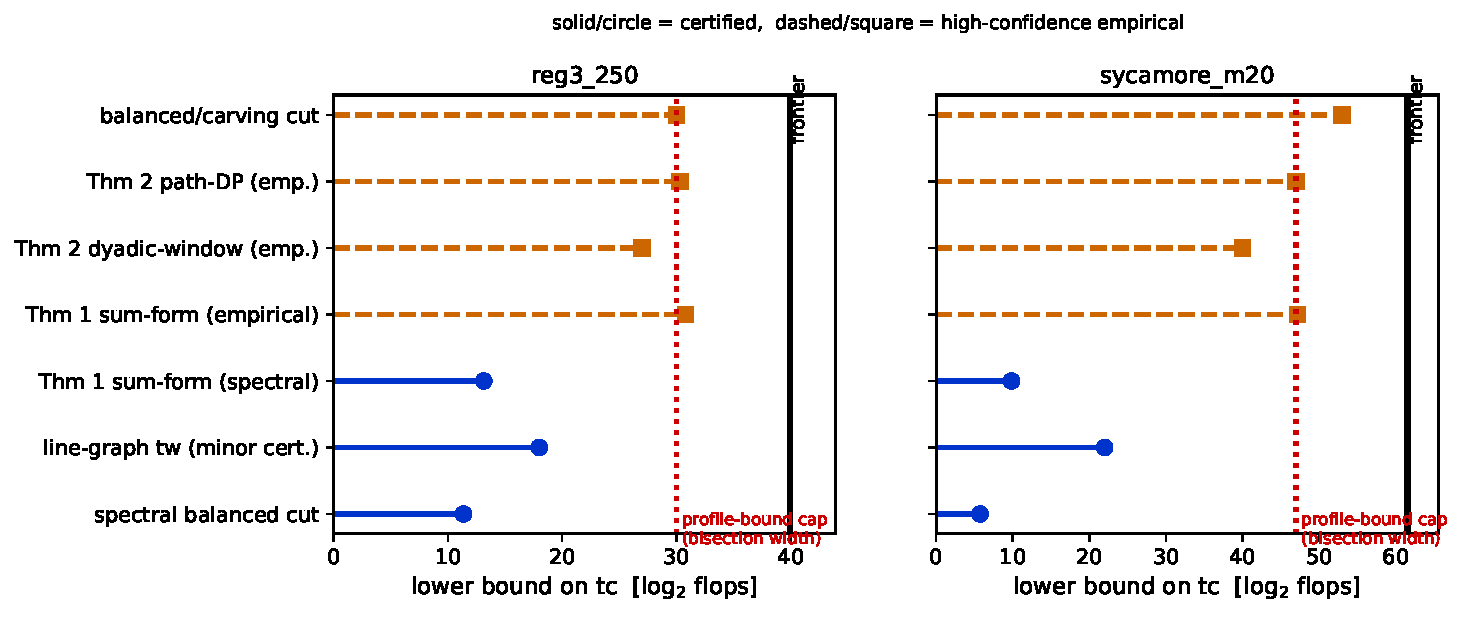
\includegraphics[width=\linewidth]{figures/fig3_bounds_ladder.pdf}
  \caption{Lower-bound ladder for both instances. Solid stems with
  circles are certified (machine-checkable certificates); dashed stems
  with squares are high-confidence empirical values (explicit cuts found
  by search; searching harder can only lower them). Every profile-based
  bound (Theorems~\ref{thm:sum} and \ref{thm:window}) is capped at the
  bisection width (dotted line, Observation~\ref{obs:cap}); only the
  balanced/carving cut exceeds it. The solid vertical line is the
  optimizer frontier.}
  \label{fig:bounds}
\end{figure}

\begin{figure}[t]
  \centering
  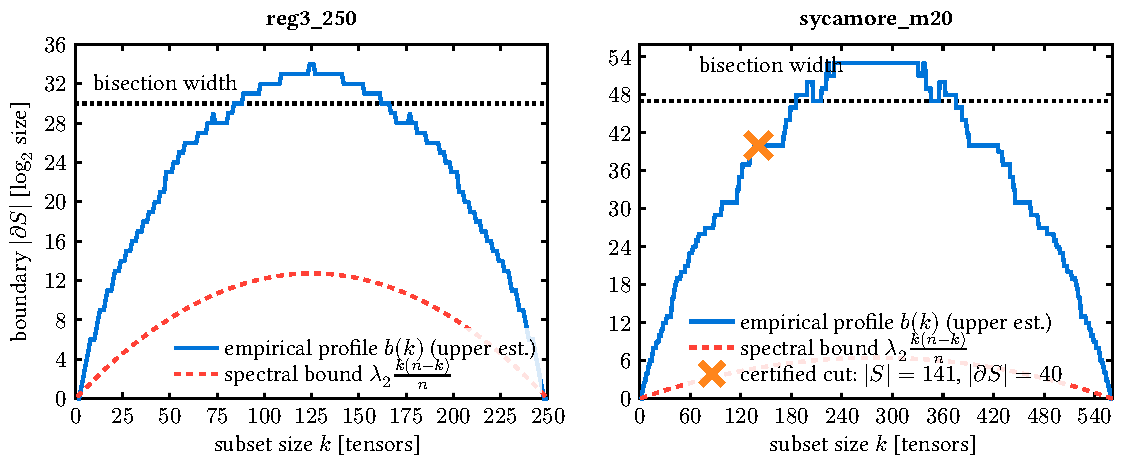
\includegraphics[width=\linewidth]{figures/fig4_isoperimetric_profiles.pdf}
  \caption{Isoperimetric profiles. The empirical profile $b(k)$ (solid)
  dips well below the bisection width (dotted) at off-center sizes; the
  certified star marks the 141-tensor sycamore\_m20 subset with boundary
  exactly 40. The spectral bound (dashed) is certified but loose. This
  dip is what caps all profile-based bounds
  (Observation~\ref{obs:cap}).}
  \label{fig:profiles}
\end{figure}

\begin{figure}[t]
  \centering
  
\includegraphics[width=\linewidth]{figures/fig5_profile_conservation.pdf}
  \caption{Cost-profile conservation at the frontier. Bars count
  contractions within $1.0$ (solid) and $2.0$ (hatched) of the largest;
  boxes give each tree's peak cost and $\tc$. Trees that lower the peak
  by one unit acquire several times more near-peak contractions at
  essentially unchanged $\tc$.}
  \label{fig:conservation}
\end{figure}

\section{Where scale changes the game}
\label{sec:scale}

At 250--561 tensors the frontier is budget-independent and
mechanism-independent; at 1000--1238 tensors neither holds
(Fig.~\ref{fig:scale}). Ninety seconds no longer suffices for
convergence, single-run variance grows to $1$--$5$ $\log_2$
units---exceeding every genuine method difference we measured---and
schedule design (continuous ramps versus restart ladders) trades early
against late quality. Our confirmation-based record protocol correctly
refuses lucky records in this regime, but symmetrically prevents real
sub-variance improvements from registering; meaningful optimizer
comparisons at scale therefore require distributional reporting
(medians over repeated runs), as practiced in
\cite{gray_2020_hyper}, and we flag our single-run scale numbers as
indicative only.

\begin{figure}[t]
  \centering
  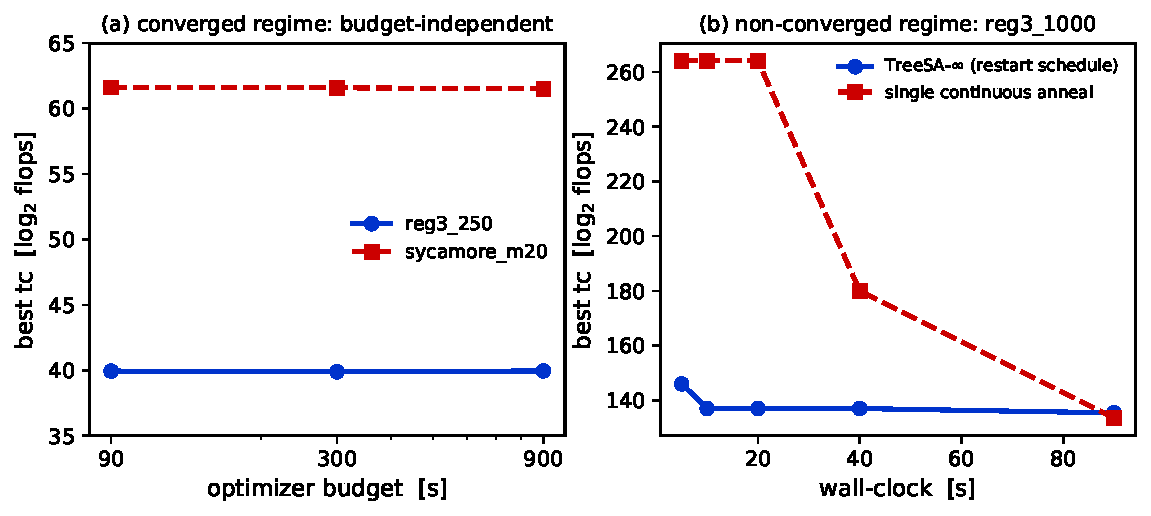
\includegraphics[width=\linewidth]{figures/fig6_scale_regimes.pdf}
  \caption{(a) Converged regime: the frontier on both benchmark
  instances is unchanged from 90 to 900 seconds. (b) Non-converged
  regime (reg3\_1000): anytime curves of the restart-ladder reference
  versus a single continuous anneal; early and late quality trade off,
  and run-to-run variance (not shown) exceeds the differences.}
  \label{fig:scale}
\end{figure}

\section{Methodology: a research loop that distrusts itself}
\label{sec:method}

The results above were produced by an autonomous research loop---31
optimizer attempts over six cycles, each in an isolated worktree with a
pre-registered hypothesis, scored by a sandboxed validator---and the
loop's central design lesson is that its most important outputs were
\emph{retractions} (Fig.~\ref{fig:timeline}). Three failure modes were
caught by the harness rather than by luck:

\emph{(i) Schedule exploitation.} The first gate (a speed-versus-baseline
bar) was passed by budget hygiene alone---anytime writes and early
termination---with no algorithmic content. The fix was structural: fold
the exploit into the reference, making schedule-only candidates score
zero by construction, and keep the exploit as a permanent negative
control.

\emph{(ii) Mis-tuned-baseline gains.} Eight mechanisms then ``beat'' the
references by up to $800\times$---until a strengthened reference (the
one-line $\scT$ fix of Sec.~\ref{sec:sctarget}) reclaimed the entire
gain. What survived was the tuning discovery itself, and the leaderboard
practice of ratcheting references to absorb every discovered
improvement, so that only genuinely new effects can score.

\emph{(iii) Instrument bias.} A failed attempt's diagnosis revealed that
the independent scorer silently rejected contraction trees deeper than
$\sim\!475$ (a recursion limit), biasing the admissible space against
exactly the deep, MPS-like trees that suit circuit instances. The scorer
was fixed, its negative-control suite re-passed, and the affected
hypothesis re-tested.

The pattern that generalizes: score only through a hardened, independent
validator (recompute everything, trust nothing the candidate reports);
maintain executable negative controls, and when a new exploit is found,
patch the harness and add the exploit to the control suite; ratchet
references so yesterday's wins are tomorrow's baselines; and treat
certified bounds, not incumbent-versus-incumbent deltas, as the quality
standard. Under this regime, every claim in this paper is either
machine-certified, or labeled high-confidence with its evidence, or was
retracted before publication---and the audit trail (per-attempt logs,
certificates, and cycle reports) ships with the code.

\begin{figure}[t]
  \centering
  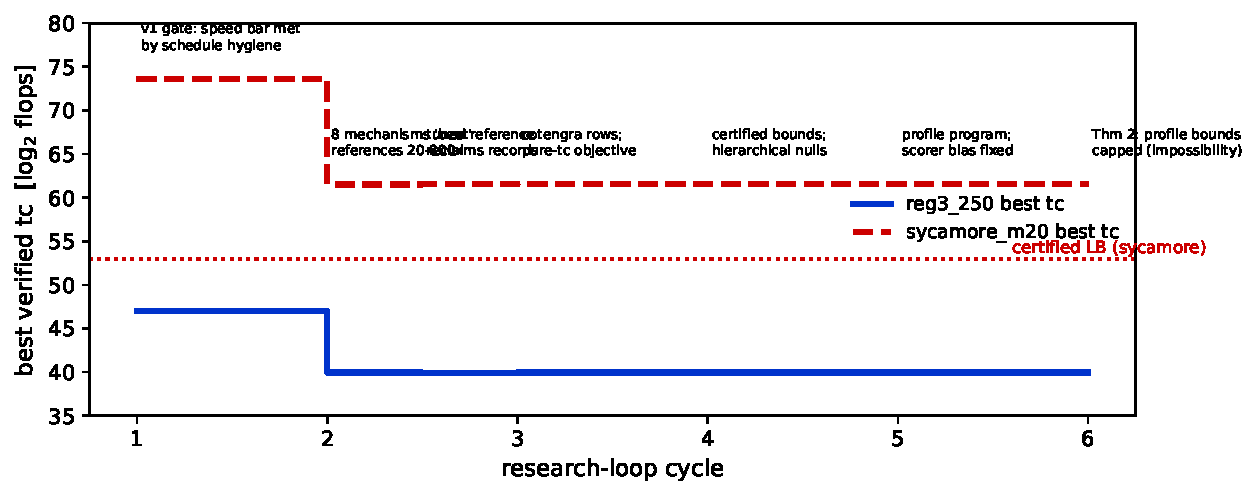
\includegraphics[width=\linewidth]{figures/fig7_methodology_timeline.pdf}
  \caption{Best verified $\tc$ over the six research-loop cycles.
  Apparent progress in cycle~2 is reclaimed by the strengthened
  reference (cycle~2.5); thereafter the frontier is flat while the
  certified picture (bounds, impossibility) grows. Annotations mark the
  three instrument-caught failure modes.}
  \label{fig:timeline}
\end{figure}

\section{How the results were found: steered autonomous research}
\label{sec:roadmap}

The findings of this paper were produced by an autonomous research loop
(machine-proposed hypotheses, isolated implementations, hardened scoring)
that was \emph{steered} by a small number of human decisions. Because the
loop retained every artifact, the causal path from the opening question to
each main result can be reconstructed exactly. Figure~\ref{fig:roadmap}
shows that path left to right: the top row quotes the steering prompts,
the middle row shows only the attempts that carried results forward
(50 of the 56 attempts served as controls, falsifications, or dead
branches feeding Sec.~\ref{sec:method}), and each arrow states why the
transition happened.

Three properties of this trajectory are worth stating explicitly.
\emph{First, every pivot was forced by a measurement, not chosen freely.}
The move from tc-optimization to the anytime axis happened because
thirteen mechanisms and a second toolchain had converged on one frontier
that was then certified locally optimal three independent ways; the move
to scale happened because time-to-frontier proved heavy-tailed at the
claim threshold; the move to global-information mechanisms happened
because every search-control variant had failed with a structural cause
while every input-level variant had won. \emph{Second, the human
contributions were few but load-bearing}: the demand for a strengthened
reference (which produced the tuning result of Sec.~\ref{sec:sctarget}),
the switch to real-provenance instances (which unlocked the
simplification pillar---the same mechanism had been correctly measured
as useless on the pre-simplified proxy two cycles earlier), and the
question ``can global information help the local search escape?'' (which
became waist surgery). \emph{Third, retests are cheap when provenance
changes}: attempt 013's null on the synthetic proxy and attempt 039's
records on the real circuit are the same mechanism measured on different
inputs, and only the pre-registered instance provenance made the
contradiction interpretable rather than embarrassing.

\begin{figure}[p]
  \centering
  \resizebox{\linewidth}{!}{%
  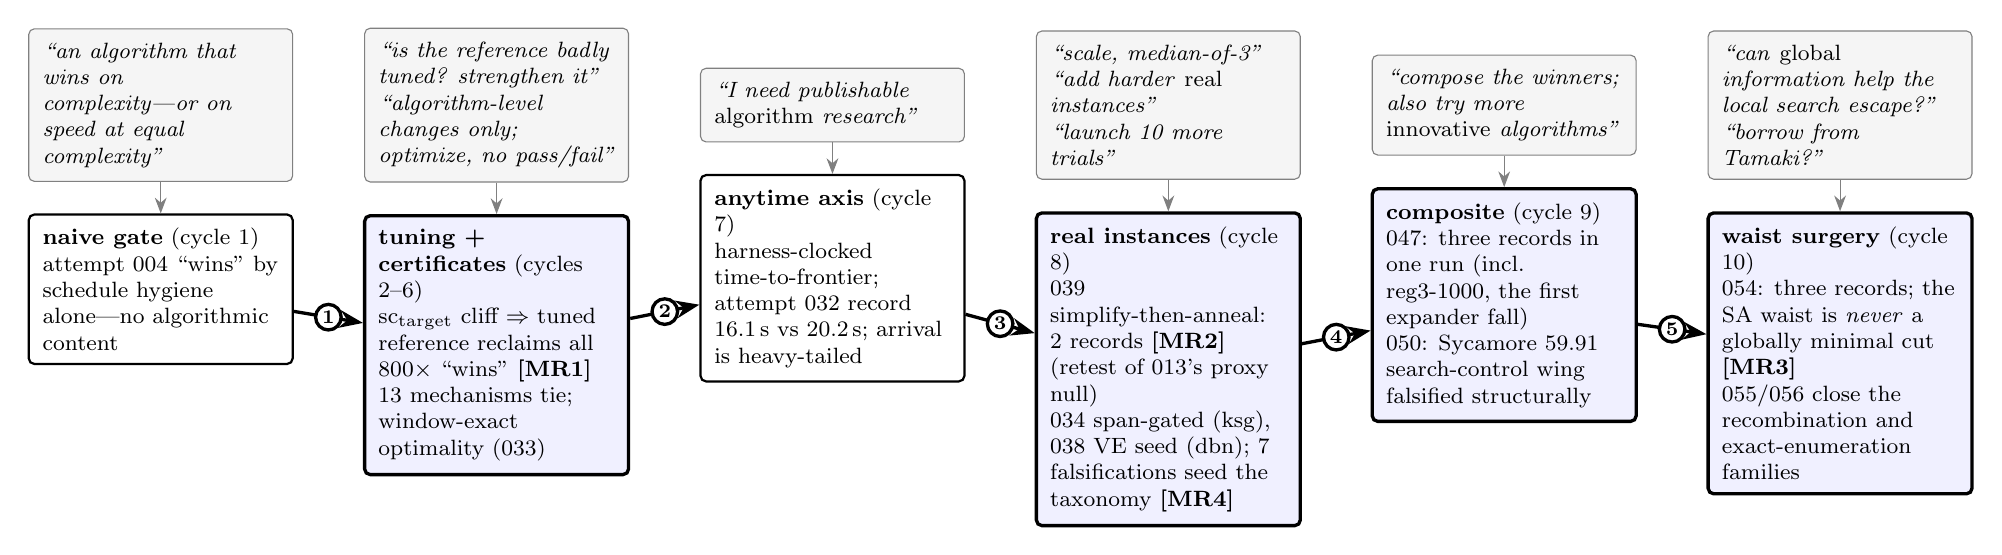
\begin{tikzpicture}[
      font=\small,
      steer/.style={draw=black!50, fill=black!4, rounded corners=2pt,
        text width=30mm, align=flush left, inner sep=5pt, font=\itshape\footnotesize},
      work/.style={draw, thick, fill=white, rounded corners=2pt,
        text width=30mm, align=flush left, inner sep=5pt, font=\footnotesize},
      res/.style={draw, very thick, fill=blue!6, rounded corners=2pt,
        text width=30mm, align=flush left, inner sep=5pt, font=\footnotesize},
      why/.style={font=\scriptsize\itshape, align=center, text width=26mm},
      flow/.style={-{Stealth[length=3mm]}, very thick},
      down/.style={-{Stealth[length=2mm]}, black!50}]

    % stage 1
    \node[steer] (s1) {``an algorithm that wins on complexity---or on
      speed at equal complexity''};
    \node[work, below=4mm of s1] (w1) {\textbf{naive gate} (cycle 1)\\
      attempt 004 ``wins'' by schedule hygiene alone---no algorithmic
      content};
    % stage 2
    \node[steer, right=9mm of s1] (s2) {``is the reference badly tuned?
      strengthen it''\\``algorithm-level changes only; optimize, no
      pass/fail''};
    \node[res, below=4mm of s2] (w2) {\textbf{tuning + certificates}
      (cycles 2--6)\\ $\scT$ cliff $\Rightarrow$ tuned reference
      reclaims all $800\times$ ``wins'' \textbf{[MR1]}\\ 13 mechanisms
      tie; window-exact optimality (033)};
    % stage 3
    \node[steer, right=9mm of s2] (s3) {``I need publishable
      \emph{algorithm} research''};
    \node[work, below=4mm of s3] (w3) {\textbf{anytime axis} (cycle 7)\\
      harness-clocked time-to-frontier; attempt 032 record
      16.1\,s vs 20.2\,s; arrival is heavy-tailed};
    % stage 4
    \node[steer, right=9mm of s3] (s4) {``scale, median-of-3''\\``add
      harder \emph{real} instances''\\``launch 10 more trials''};
    \node[res, below=4mm of s4] (w4) {\textbf{real instances} (cycle 8)\\
      039 simplify-then-anneal: 2 records \textbf{[MR2]} (retest of
      013's proxy null)\\ 034 span-gated (ksg), 038 VE seed (dbn);
      7 falsifications seed the taxonomy \textbf{[MR4]}};
    % stage 5
    \node[steer, right=9mm of s4] (s5) {``compose the winners; also try
      more \emph{innovative} algorithms''};
    \node[res, below=4mm of s5] (w5) {\textbf{composite} (cycle 9)\\
      047: three records in one run (incl.\ reg3-1000, the first
      expander fall)\\ 050: Sycamore 59.91\\ search-control wing
      falsified structurally};
    % stage 6
    \node[steer, right=9mm of s5] (s6) {``can \emph{global} information
      help the local search escape?''\\``borrow from Tamaki?''};
    \node[res, below=4mm of s6] (w6) {\textbf{waist surgery} (cycle 10)\\
      054: three records; the SA waist is \emph{never} a globally
      minimal cut \textbf{[MR3]}\\ 055/056 close the recombination and
      exact-enumeration families};

    \foreach \i in {1,...,6} {\draw[down] (s\i) -- (w\i);}

    \draw[flow] (w1) -- node[circle, draw, fill=white, inner sep=1pt,
      font=\scriptsize\bfseries] {1} (w2);
    \draw[flow] (w2) -- node[circle, draw, fill=white, inner sep=1pt,
      font=\scriptsize\bfseries] {2} (w3);
    \draw[flow] (w3) -- node[circle, draw, fill=white, inner sep=1pt,
      font=\scriptsize\bfseries] {3} (w4);
    \draw[flow] (w4) -- node[circle, draw, fill=white, inner sep=1pt,
      font=\scriptsize\bfseries] {4} (w5);
    \draw[flow] (w5) -- node[circle, draw, fill=white, inner sep=1pt,
      font=\scriptsize\bfseries] {5} (w6);
  \end{tikzpicture}}
  \caption{The research roadmap, left to right. Top row (grey): the
  human steering prompts, essentially verbatim. Bottom row: the
  result-carrying attempts only (shaded boxes contain main results);
  50 of 56 attempts are controls and falsifications that feed the
  mechanism taxonomy and Sec.~\ref{sec:method}. Each numbered arrow is a
  transition forced by a measurement: (1) the gate was passed without an
  algorithm, so the gate was hardened and references ratcheted; (2) tc
  saturated and was certified locally optimal, so the objective axis
  changed to arrival time; (3) speed gains sat at the confirmation noise
  floor while scale budgets were non-converged, so the regime changed;
  (4) the winning mechanisms proved complementary, so they were composed
  while exploration continued; (5) every win injected global information
  as \emph{input} while every search-control variant failed, so global
  information was aimed directly at the local search's blind spot---the
  dominant cut.}
  \label{fig:roadmap}
\end{figure}

\section{Conclusions}
\label{sec:conclusions}

On standard contraction benchmarks under a fixed matched-budget protocol,
we found that (1) the dominant practical effect is a shipped default: an
aspirational memory target costs $20\times$--$800\times$ in flops, is
harmful in one direction only, and is fixed by removing the target unless
a physical memory budget exists; (2) with that fixed, thirteen search
mechanisms and two independent toolchains converge on a single,
budget-independent frontier that simulated-annealing refinement---from
either toolchain---reaches and hyper-optimization alone does not; and
(3) on the circuit proxy the frontier is certifiably width-optimal, the
optimum lies in $[53, 61.544]$, and no bound computable from the
isoperimetric profile can close the interval further
(Observation~\ref{obs:cap})---the remaining gap is jointly-nested-cut
structure plus an apparently conserved log-sum residual.

The implications we would highlight: defaults in shipped optimizers
deserve adversarial benchmarking, because a parameter can outweigh a
decade of mechanism design; certified references, even partial ones,
change what optimizer comparisons mean; and carving/branch-width-type
machinery is the right target for future bound development, as profile
methods are provably exhausted. Natural next steps are carving-width
lower-bound certification, variance-aware protocols for large instances,
physical circuit instances in place of proxies, and heterogeneous bond
dimensions, where the weighted problem is largely unexplored.

\section*{Code and data availability}
The optimizer (omeco), the validation harness, all certificates
(treewidth minors, cut sets, and their verification scripts), per-attempt
logs, and the cycle reports of the research loop are available in the
project repository.

\section*{Acknowledgments}
The research loop was orchestrated with LLM-based agents under
pre-registered hypotheses and independent validation; all certified
claims were verified by machine-checkable artifacts independent of any
agent output.

\bibliographystyle{plain}
\bibliography{references}

\end{document}
